%%%%%%%%%%%%%%%%%%%%%%%%%%%%%%%%%%%%%%%%%%%%%%%%%%%%%%%%%%%%%%%%%%%%%%%%
\section{Assignment}
\subsection{Overview}

\subsection{Results}

Data was downloaded from \url{http://sidc.be/silso/datafiles} and \url{ftp://ftp.ngdc.noaa.gov/STP/GEOMAGNETIC_DATA/INDICES/KP_AP}, year 2003, and the data format was checked.
\subsection{Discussion}




%%%%%%%%%%%%%%%%%%%%%%%%%%%%%%%%%%%%%%%%%%%%%%%%%%%%%%%%%%%%%%%%%%%%%%%%
\section{Assignment}
\subsection{Overview}
In this Assignment we modify the settings for the model IRI2001 with the data gathered in the previous task, and re-run the IRI2001 model.
The results are then compared to the default case.
\subsection{Results}

\begin{figure}[h]
	\centering
	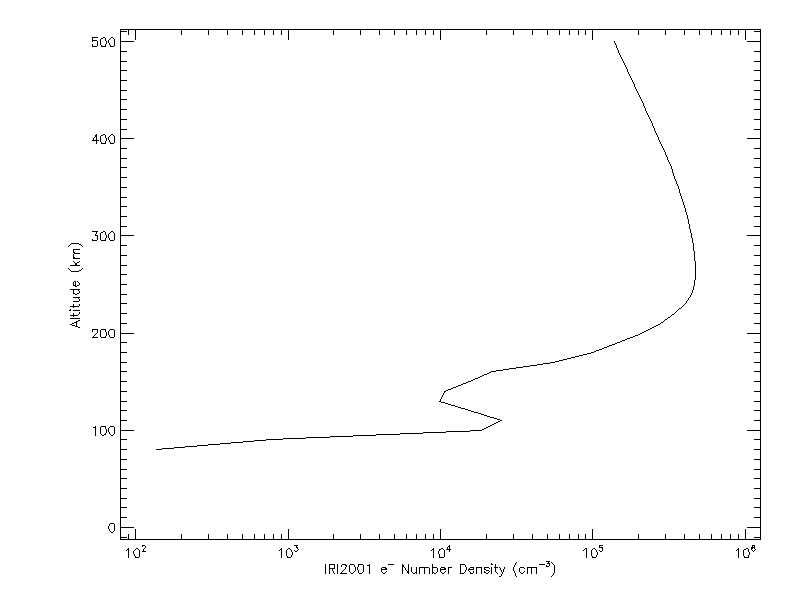
\includegraphics[width=\linewidth]{images/E_number_density_plot1}	
	\caption{Electron number density Plot Old}
	\label{fig:ass2Plot1}
\end{figure}
\begin{figure}[h]
	\centering
	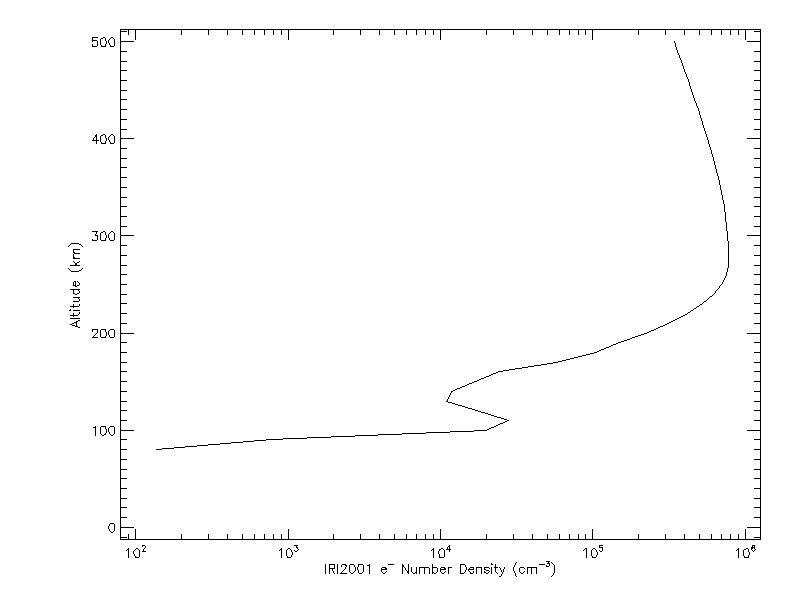
\includegraphics[width=\linewidth]{images/E_number_density_plot2}	
	\caption{Electron number density Plot New}
	\label{fig:ass2Plot2}
\end{figure}

\subsection{Discussion}
For the default case, the number density is much lower at higher altitudes than it is for the corrected value, for example: at an altitude of approx. 500km the number density is around $10^{5.05}$, whereas for the latter case the number density at 500km is approx. $10^{5.2}$.





%%%%%%%%%%%%%%%%%%%%%%%%%%%%%%%%%%%%%%%%%%%%%%%%%%%%%%%%%%%%%%%%%%%%%%%%
\section{Assignment}
\subsection{Overview}
The model IRI2001 used in Assignment 1 is used again. The year shall stay the same, but other parameters as Day of Year, the daily $F_{10.7}$ and the 12 month average sunspot number are changed.
\subsection{Results}
We used the following values for the parameters to be changed
\todo{make a table here or something}

year 2003
SD:7.1
average sunspot number 99.3
Selecting Day 1

\begin{figure}[h]
	\centering
	\includegraphics[width=\linewidth]{images/ass3plot1}	
	\caption{Electron number density with standard deviation}
	\label{fig:ass3Plot1}
\end{figure}

The sunspot number parameter has almost no effect at lower altitudes, however at approx. 250km the electron number density starts to vary. The lower the sunspot number the lower the electron number density at each respective altitude above 250km.
\todo{insert plot here km/e-}

2. The electron number density varies on a diurnal basis, but only very minutely. 

3. Comparing Winter and Summer (day 1 and day 181), the electron number density varies on a larger scale.
\subsection{Discussion}



%%%%%%%%%%%%%%%%%%%%%%%%%%%%%%%%%%%%%%%%%%%%%%%%%%%%%%%%%%%%%%%%%%%%%%%%
\section{Assignment}
\subsection{Overview}
\subsection{Results}
Since the given latitude and longitude are located in the auroral region, and 2003 was close to a maximum of the sun's 11-year cycle, the IRI2001 Model is not suitable as this is not magnetically-quite region.
\subsection{Discussion}



%%%%%%%%%%%%%%%%%%%%%%%%%%%%%%%%%%%%%%%%%%%%%%%%%%%%%%%%%%%%%%%%%%%%%%%%
\section{Assignment}
\subsection{Overview}
\subsection{Results}
\todo{todo}
D-Layer below 90

E 90-130

F1-130
\begin{figure}[h]
	\centering
	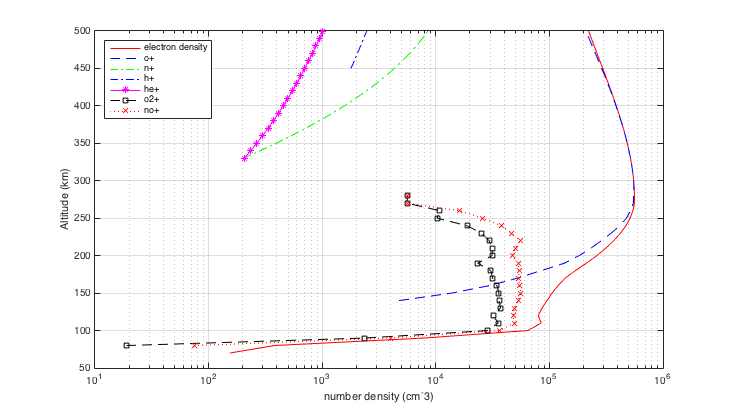
\includegraphics[width=\linewidth]{images/ass5_properties_plot}	
	\caption{bla}
	\label{fig:ass5Plot}
\end{figure}


\subsection{Discussion}

